\section{Part 2}

\subsection{Inference Algorithms}
To be able to do proper inference on top of the HMM, we need to exploit the conditional independencies in the graph and try to cluster some of the variables to perform message passing on those clusters. The clustering we will consider is the following\\
\hspace{1cm}\\
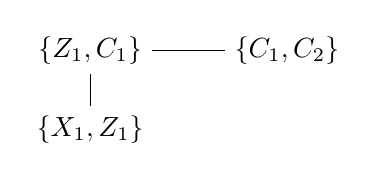
\begin{tikzpicture}
    % Define nodes
    \node (X1) at (0,0) {$\{X_1,Z_1\}$};
    \node (Z1) at (0,1) {$\{Z_1,C_1\}$};
    \node (C1) at (2.5,1) {$\{C_1,C_2\}$};
    
    % Draw edges
    \draw (X1) -- (Z1);
    \draw (Z1) -- (C1);
\end{tikzpicture}

We will be performing message passing on HMM using the clique tree in \cref{fig:Clique Tree}
\begin{figure}
\centering
  \includegraphics[width=0.9\textwidth]{latex/figures/clique_tree.pdf}
  \caption{Data generation visualization.}
  \label{fig:Clique Tree}
\end{figure}

We denote the cliques $\{C_i,C_{i+1}\}$ as clique $A_i$, for $i=1,...,T-1$, $\{C_i, Z_{i1},...,Z_{in}\}$ as clique $B_i$, for $i=1,...,T$, and $\{ X_{i1},...,X_{in},Z_{i1},...,Z_{in}\}$ as clique $B_i$, for $i=1,...,T$

\subsection{Test of Inference Algorithms}

\subsection{Application of Inference Algorithms on Data}

